\documentclass{article}
\usepackage{graphicx} % Required for inserting images
\usepackage{tikz}
\usepackage{natbib}
\usepackage{array}
\usepackage{amsmath}
\usepackage{amssymb}
\usepackage{lscape}

\usepackage{pgfplots}


\usetikzlibrary{shapes.geometric, arrows,fillbetween}

\title{U1}
\author{Rodriguez González José Adrián }
\date{August 2024}

\begin{document}

\maketitle
\tikzstyle{startstop} = [rectangle, rounded corners, minimum width=3cm, minimum height=1cm,text centered, draw=black, fill=red!30]
\tikzstyle{process} = [rectangle, minimum width=1.5cm, minimum height=1.5cm, text centered, draw=black, fill=orange!30,text width=3cm]
\tikzstyle{decision} = [diamond,  minimum width=1.5cm, minimum height=1.5cm, text centered, draw=black, fill=green!30,text width=2cm]
\tikzstyle{arrow} = [thick,->,>=stealth]
\section{Abstract}
In data analysis we need to understand that every analysis problems requires its own time before to create a predictive model. This is because we need to verify if our model would it be useful.
We have two problems to practice that it has been learned about data analysis. As first checkout it'll be a simple dataset that only have two features \(x and y\). So at the first sight seems to be quick but before to create a predictive model, it'll be required to take a look into the data as first step. And also, we got another case about predicte the price of cars.
\section{Introduction}
With the objective to checkout how does it work the linear regression and look out for troubles on the real life. It has been presented two datasets. The first one consist in sintetic data.
And the second one is related wth the prices of cars, and involves several features and the main objective on these datasets is to create a predictor that may predict future data.
\section{Related works}
Some of the related works(by now, I'll just let some of the books and the docoumentation that I could  to see)
\begin{center}
  \begin{tabular}{|m{2.5cm}|m{2.5cm}|m{2.5cm}|m{2.5cm}|m{2.5cm}|}
    \hline
    Article & Year & Techniques & Data & Results \\ \hline
    Consumers' preferences on the Swiss car market: A revealed preference approach& 2019&hedonic pricing approach and linear regression& Were obtained on the auto-Schweiz website&How lastly the costumers have been prefered lighter cars than heaviear despite the increasing of the weight cars and how it is an important factor for the costumer the efficence on the fuel consumtion\\
    \hline
    İkinci El Otomobil Fiyat Artışına Etki Eden Faktörlerin Yapısal Eşitlik Modeli ile Tespit Edilmesi: Van İli Örneği( Determination of the Factors Affecting the Used Car Price Increase with the Structural Equation Model: The Case of Van Province) & 2023 & AFA, and structured equation model& Were obtaind due to surveyrs on the province of Van & It has been found how the several features as economics, marketing, strategies and supplying are correlated with the amount of prices, however the economics are is stronger against the other factors\\
    \hline
    % Aquí puedes agregar más filas de datos
  \end{tabular}
\end{center}
\section{Methods and materials}
The material used for this analysis were the usage of python and its libraries for data analysis and machine learning:
\begin{itemize}
  \item Numpy: For mathematical calculations
  \item Pandas: For handle datasets 
  \item scipy: to evaluate statistical parameters
  \item Scikit-learn: to train our model and check more parameters related with the model chosen.  
\end{itemize}
The methodology followed it's the mix of scientific methodology with the abstractacion for a data scientist. 
\begin{itemize}
  \item Obtain the data
  \item Make an exploration into the data.
  \item Check various parameters from the dataset.(These parts involves most of the section of exploratory anaylisis, as also, this step gives several hypothesis to check out at the dataset)
  \item Now that we have our Hypothesis planted, and also, with the help of th last step that it can be plotted the data. Now it'll be cleaned the data, and for this section it incquires in several steps
  \item \begin{itemize}
    \item Hypothesis proposal
    \item Transformations (logarithm, square, box-cox, capping and flooring)
    \item Check the metrics of skewness, $R^2$, $MSE$,$RMSE$ 
    \item Make the model of linear regression 
  \end{itemize}
  \item check its metrics
  \item Propouse another hypothesis.
\end{itemize}
Also, the main models that has been studied were Linear regression and Knn regresor
\subsection{Linear regresion}
When we try to represent something complex it is usual that it has to be create a structure that simplifies the process however, it must contain the enough data and values that can approachthe behaviour of phenomen. In science areas, it is commonnly called model.
A model can explain a complex phenomen in simple terms that can be easy handled and understandable.
One of the most simplest models that exist on data science is the linear regression. 
Knowing:
$$f:\mathbb{R} \rightarrow \mathbb{R} $$
we have:
$$f(x)=mx+b$$


\begin{figure}[h]
  \centering
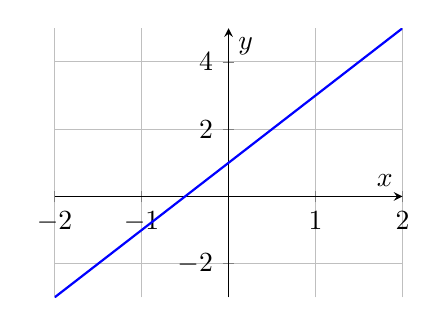
\begin{tikzpicture}
    \begin{axis}[
        axis lines = middle,
        xlabel = \(x\),
        ylabel = {\(y\)},
        samples = 100,
        domain=-2:2,
        grid=both,
        width=6cm,
        height=5cm,
    ]
    \addplot[blue, thick] {2*x + 1};
    \end{axis}
\end{tikzpicture}
  \caption{An example of a lineal function}
  \label{fig:example2}
\end{figure}


This is a linear function(Figure \ref{fig:example2}),  one of the simpliest functions that can be viewed on calculus, sometimes a simple phenomen can be viewed without getting in a huge amount of complexity and could be described with simple models, and when we have a problem or a situation in the reality when we need to create a machine hat can predict future data, what can we do?
In those cases, as it has been portrayed, a linear function can be used as a mathematical feature that attempts to fit on the data.
\begin{figure}[h]
\centering
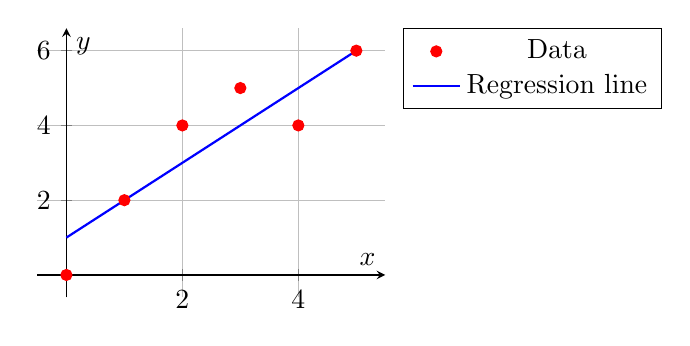
\begin{tikzpicture}
  \begin{axis}[
      axis lines = middle,
      xlabel = \(x\),
      ylabel = {\(y\)},
      grid = both,
      width = 6cm,
      height = 5cm,
      enlargelimits = true,
      legend style={at={(1.05,1)}, anchor=north west},
  ]
  % Puntos de datos
  \addplot[
      only marks,
      mark=*,
      color=red,
  ] table {
      0 0
      1 2
      2 4
      3 5
      4 4
      5 6
  };
  
  % Línea de regresión (calculada)
  \addplot[
      domain=0:5, 
      samples=100, 
      color=blue, 
      thick
  ] {x + 1};
  
  \legend{Data, Regression line}
  
  \end{axis}
\end{tikzpicture}
  \caption{A simple example of a lineal regression}
  \label{fig:example3}
\end{figure}
Despite that nowadays exist several types of models that can predict future data, lineal regression as it is one of the simpliest due to it just use a mathematical function that is easy to use, a lot of new models can be tested with a contraposition of lineal regression.
So, the Lineal regression is described as 
$$y=\beta_0x+\beta_1+e$$
$\beta_0$ it is the slope and $\beta_1$ is the intercept. And e is the error tha exist on the model.

However it'll be required to know some metrics that will help us to find out how efficent is our model and to know the error that we have in our model too
\begin{itemize}
  \item $R^2$: This metric can measure how much the model can describe the phenomen. The $R^2 \in [0,1]$ and if the model tends to 1 the model can describe better the phenomen and can be more precise in the predictions.
  \item $MSE$ and $RMSE = $ Are metrics that measure the distance between the value predict against the real value.
  $$MSE=\frac{1}{n}\Sigma^{n}_{i=1}(y_i-\hat{y}_i)^2 $$
    $$RMSE=\sqrt{\frac{1}{n}\Sigma^{n}_{i=1}(y_i-\hat{y}_i)^2} $$
    The difference between MSE and RMSE are that MSE is susceptible to detect outliers values due to the nature of a square function, and also it helps to know the variance that we got in our model. Nevertheless, RMSE use the same scale of the values and want to measure the error as it is on the data.

\end{itemize}

\subsection{Knn model}
It consist in to look out on the data and predict a value according to the vecinity of the values nearest from the data that is presented. Knn presents two basci hyperparameters, the first one is the number of vecinity and the second is the type of distante that it'll be chosen.
Knn model has some different parameters if we measure it as classifier. However at this case it'll be used the Knn model as a regressor, so it'll be usable the metrics that it has been described before.
(figure \ref{fig:example4})
\begin{figure}[h]
  \centering
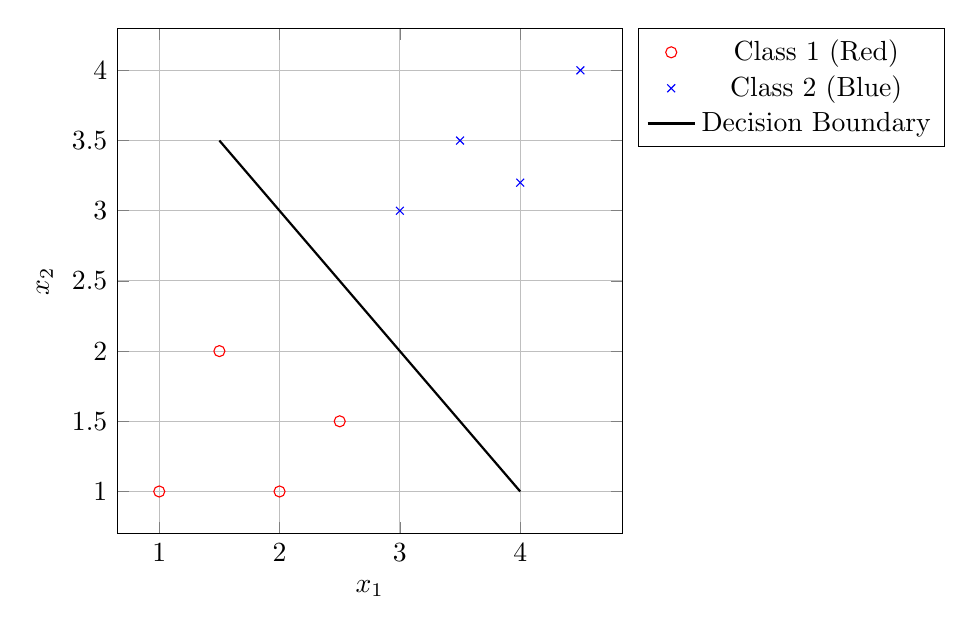
\begin{tikzpicture}
  \begin{axis}[
      width=8cm, height=8cm,
      xlabel={$x_1$},
      ylabel={$x_2$},
      grid=major,
      legend pos=outer north east,
      domain=0:5,
      samples=100
  ]
      % Define the coordinates of two classes
      \addplot[only marks, red, mark=o] plot coordinates {(1,1) (1.5,2) (2,1) (2.5,1.5)};
      \addplot[only marks, blue, mark=x] plot coordinates {(3,3) (3.5,3.5) (4,3.2) (4.5,4)};
      
      \addlegendentry{Class 1 (Red)}
      \addlegendentry{Class 2 (Blue)}
      
      % Plot decision boundary (simplified for K=1)
      \addplot [domain=1.5:4, samples=2, thick,range=3:1] {-x+5};
      \addlegendentry{Decision Boundary}
      
  \end{axis}
\end{tikzpicture}

  \caption{A simple example of knn regressor}
  \label{fig:example4}
\end{figure}
After knowing the main features that were used at this study, let's look out for the process that has been followed. As it'll have seen, the process aims to use the scientifical method, however, with the feauters of a data analyst

\begin{tikzpicture}[node distance=2cm]
  
  % Nodes
  \node (start) [startstop] {Read the datasets};
  \node (process1) [process, below of=start] {Processing the data};
  \node (proccess2)[process, right of=process1, xshift=2cm]{Data exploration};
  \node (proccess3)[process, right of=proccess2, xshift=2cm]{Finding descriptive values and NaNs};
  \node (proccess4)[process, below of=proccess3]{Applying transformations};
  \node (proccess5)[process, left of=proccess4, xshift=-2cm]{Comparate with metrics and plotting};
  \node (proccess6)[process, left of=proccess5, xshift=-2cm]{Create a regressor model and checking out the relevant metrics};
 
  \node (decision1) [decision, below of=proccess6, yshift=-2cm] {The model may be upgraded it?};
  \node (process2a) [process, below of=decision1, xshift=-4cm] {Check and reviewing with different perspectives};
  \node (decision2) [decision, below of=decision1, xshift=4cm] {My model is underfitted or overfitted?};
  \node (process3a)[process, below of=proccess6, xshift=4cm]{Comparate it with Knn model};
  \node (process4a)[process, below of=decision2, xshift=4cm]{Make their confidence intervals and propose the model};
  \node (stop) [startstop, below of=process2a, yshift=-1cm, xshift=3cm] {Stop};
  
  % Arrows
  \draw [arrow] (start) -- (process1);
  \draw [arrow] (proccess6) -- (decision1);
  \draw [arrow] (process1) -- (proccess2);
  \draw [arrow] (proccess2) -- (proccess3);
  \draw [arrow] (proccess3) -- (proccess4);
  \draw [arrow] (proccess4) -- (proccess5);
  \draw [arrow] (proccess5) -- (proccess6);
  \draw [arrow] (proccess6) --  (process3a);
  \draw [arrow] (process3a) --  (decision1);
  
  \draw [arrow] (decision1) -- node[anchor=east,yshift=0.2cm] {Yes} (process2a);
  \draw [arrow] (decision1) -- node[anchor=west,yshift=0.2cm] {No} (decision2);
  \draw [arrow] (decision2) -- node[anchor=west,yshift=-0.2cm] {Yes} (process2a);
  \draw [arrow] (decision2) -- node[anchor=west,yshift=0.2cm] {No} (process4a);
  \draw [arrow] (process2a) |- (process1);
  \draw [arrow] (process4a) |- (stop);
  \end{tikzpicture}
  
  \begin{figure}[h]
  \caption{The procedural followed at the investigation}
  \label{fig:diagram}
  
\end{figure}

These were the main steps followed at the work. The part of reading some material and check information from several sources, is mainly the first step before to begin the work. However if there's something missing when the hypothesis are covered, it'll be useful to look for more sources to create other hypothesis.

\section{Data analysis}
\subsection{first dataset}
The first data analysis that has been studied was the dataset with sintetic data. As it had been mentioned, following the scientifical methodology we look for the data and it started with a data exploration.
It obtained the following values 
\begin{center}
  \begin{tabular}{|c|c|c|}
    \hline
   parameter & y & x \\ \hline
   number of values & 506.000000 & 506.000000\\
   mean  &  22.528854  &  3.613524\\
   std   &   9.182176  &  8.601545\\
   minimum   &   5.000000  &  0.006320\\
   percentile $25$   &  17.025000  &  0.082045\\
   percentile $50$   &  21.200000  &  0.256510\\
   percentile $75$   &  25.000000 &   3.677083\\
   maximum   &  50.000000  & 88.976200\\
   \hline
    % Aquí puedes agregar más filas de datos
  \end{tabular}
\end{center}
Now that we have assured that the data are completed we can see the value of the mean and the 50 percentile are quited different, mostly on the variable x, it requires to be cleaned the data. Nevertheless, it is useful to check the correlation with variable x to y too.
The correlation matrix resulted on 
\begin{center}
  \begin{tabular}{|c|c|c|}
    \hline
      & y & x  \\ \hline
     y&  1.000000 & -0.389582 \\
     x & -0.389582  & 1.000000 \\
     \hline
    % Aquí puedes agregar más filas de datos
  \end{tabular}
\end{center}
\begin{figure}[h]
  \centering
  \includegraphics[width=0.35\textwidth]{data1_plot1.png}
  \caption{E}
  \label{fig:ejemplo}
\end{figure}


The correlation is quite low between x,y. That means that it'll be hard to find a relation with the x and y with linear regression.
And also, something that we can notice with the plots that they are not normally distribuitted. The x-axis it seems more a exponential distribution than normal.
Other way to demostrate it could making a hypothesis test and comprobating it with a Shapiro-walk; it consist to propose a null hypothesis, that if the value of statistic is closer to 1 or great, it will reject the hypothesis, therefore the distribution doesn't follow a normal distribution. By other hand if we encounter a value smaller it will indicate is that probably the distribution follows a normal dsitrbution. And also we have de p value that if is greater than 0.05 will indicate that is a normal distribution, in the oppostive way it is a non-normal distribution.
The test concluded with a distribution of  $4.85*10^-28$ so it is not a normal distribution.
At this point we can choose several ways to follow
\begin{itemize}
  \item Trying to normalizing
  \item Trying with models more associated with exponential distributions or models that will no depend on the distribution.
  \item Infere with other features
\end{itemize} 
Due to the objectives of the work, the first attempt it'll be used.
At this dataset has been followed 4 approaches to look the efficence of methods at the cleaning of the data.
However, it has been tested several types of transformations to check out if it'll be more useful the logarithm transformation according with the parameter of skew 

\begin{center}
  \begin{tabular}{|c|c|c|}
    \hline
     type-skew & x & y  \\ \hline
     original& 5.223148798243851&1.1109118502479587\\
     log&1.2692005882725572&-0.24563979611568673\\
     sqrt&2.024382103123676&0.4381663127860419\\
     1/x&-0.5772191040682719&1.9393215717506038\\
     box-cox&0.093649&\dots\\
     outliers&0.40335&1.058543\\
      \hline
    % Aquí puedes agregar más filas de datos
  \end{tabular}
\end{center}
It could seems some techniques are better however logarithm tranformation has a better resolution in the skew of both variables.    
\subsection{first method}
The fisrt approach to make a model was transforming with logarithm and making a cross validation
\begin{figure}[h]
  \centering
  \includegraphics[width=0.35\textwidth]{model_1.png}
  \caption{Lineal regression}
  \label{fig:example_1}
\end{figure}
And therefore it was contrasted with the Knn model, getting the next values

\begin{center}
  \begin{tabular}{|c|c|c|}
    \hline
     metric & Lineal regression & Knn \\ \hline
     $R^2$l& 35.488840060699256\%&43.57\\
     MSE&0.09611374428381783&0.11904\\
     RMSE&0.30971201639466434&0.33166\\
     \hline
    % Aquí puedes agregar más filas de datos
  \end{tabular}
\end{center}
The model has been contrasted with both models and with the same cleaned data, as also trained at the same way respectively at the model 
However, the Lineal regressor has been predicting the data within the confidence.
For example, it added a value x on 2.3 and the result in y is 2.7534 
The confidence value on 95\% interval is  from $(2.172214750599946, 3.334689169873629)$
and is has been seen the value was fitted correctly.
\begin{figure}[h]
  \includegraphics[width=0.35\textwidth]{data2_plot.png}
  \caption{Lineal regresion with the intervals set}

  \label{fig:example_intervals}
\end{figure}
However it has been made a generalized model to linear regression in a set of dots (fig\ref{fig:example_intervals})
The equation for this model is 
$$y=-0.21773690693332431x+3.2542468461834333$$
\subsection{second method}
The second approach it consisted to just transforming the value with logarithm without CV 5x2
\begin{center}
  \begin{tabular}{|c|c|c|}
    \hline
     metric & Lineal regression & Knn \\ \hline
     $R^2$& 15.0589474050694\%&22.562569548739275\%\\
     MSE&0.1127456496305317&0.11904364904719832\\
     RMSE&0.3357761897909554&0.33166\\
     \hline
    % Aquí puedes agregar más filas de datos
  \end{tabular}
\end{center}
\subsection{third method}
The outliers were fixed with capping and flooring methos using the median
\subsection{fourth method}
The last methods were used at this model

The methods were contrasted by the simplest model and also the intervals were obtained, however that section it comprehends the results discussion

And one of the most important things that iat has been obtained is this table that compiles all the metrics and parameters that has been obtained
\begin{table}[h]
  \centering
  \small % Cambia el tamaño de la fuente aquí
  \begin{tabular}{|l|l|l|}
  \hline
  \textbf{Métrica} & \textbf{model1} & \textbf{model2} \\
  \hline
  $R^2$ & 36.9\% & 39.9\% \\
  \hline
  MSE & 0.0961 & 0.1127 \\
  \hline
  RMSE & 0.3097 & 0.3358 \\
  \hline
  EQUATION & $y=-0.2177x+3.2542$ & $y=-0.2479x+3.2824$ \\
  \hline
  Adjusted $R^2$ & 36.7\% & 39.8\% \\
  \hline
  F-statistic & 147.1 & 267.1 \\
  \hline
  $P(F-statistic)$ & 5.97e-27 & 2.11e-46 \\
  \hline
  Log-Likelihood & -50.079 & -91.384 \\
  \hline
  AIC & 104.2 & 186.8 \\
  \hline
  BIC & 111.2 & 194.8 \\
  \hline
  std error & const=0.024, x=0.018 & const=0.019, x=0.015 \\
  \hline
  $\sigma$ & const=135.161, x=-12.128 & const=170.036, x=-16.343 \\
  \hline
  $P>\|t\|$ & const: 0.000, x: 0.000 & const: 0.000, x: 0.000 \\
  \hline
  Confidence Intervals & const=[3.2068, 3.3017], x=[-0.2531, -0.1824] & const=[3.2444, 3.3203], x=[-0.2777, -0.2181] \\
  \hline
  Omnibus & 41.738 & 37.308 \\
  \hline
  Prob(Omnibus) & 0.000 & 0.000 \\
  \hline
  Jarque-Bera (JB) & 64.331 & 64.192 \\
  \hline
  Prob(JB) & 1.07e-14 & 1.15e-14 \\
  \hline
  Skew & 0.960 & 0.581 \\
  \hline
  Kurtosis & 4.553 & 4.570 \\
  \hline
  Durbin-Watson & 0.983 & 1.902 \\
  \hline
  Condition Number & 2.26 & 2.16 \\
  \hline
  \end{tabular}
  \caption{Comparación de los modelos 1 y 2}
  \label{tab:modelos12}
  \end{table}
  
  \begin{table}[h]
  \centering
  \small % Cambia el tamaño de la fuente aquí
  \begin{tabular}{|l|l|l|}
  \hline
  \textbf{Métrica} & \textbf{model3} & \textbf{model4} \\
  \hline
  $R^2$ & 33.8\% & 37.1\% \\
  \hline
  MSE & 0.014957 & 0.0807 \\
  \hline
  RMSE & 0.12224 & 0.2839 \\
  \hline
  EQUATION & $y=-0.30537x+1.85673$ & $y=-0.2052x+3.2467$ \\
  \hline
  Adjusted $R^2$ & 33.5\% & 36.8\% \\
  \hline
  F-statistic & 128.2 & 147.8 \\
  \hline
  $P(F-statistic)$ & 2.76e-24 & 4.72e-27 \\
  \hline
  Log-Likelihood & 181.27 & -32.091 \\
  \hline
  AIC & -385.5 & 68.18 \\
  \hline
  BIC & -351.5 & 75.25 \\
  \hline
  std error & const=1.8567, x=-0.3054 & const=0.022, x=0.017 \\
  \hline
  $\sigma$ & const=0.015, x=0.027 & const=144.464, x=-12.159 \\
  \hline
  $P>\|t\|$ & const: 0.000, x: 0.000 & const: 0.000, x: 0.000 \\
  \hline
  Confidence Intervals & const=[1.8279, 1.886], x=[-0.3584, -0.2522] & const=[3.2024, 3.2909], x=[-0.2384, -0.1719] \\
  \hline
  Omnibus & 40.637 & 35.555 \\
  \hline
  Prob(Omnibus) & 0.000 & 0.000 \\
  \hline
  Jarque-Bera (JB) & 56.377 & 46.953 \\
  \hline
  Prob(JB) & 5.73e-13 & 6.37e-11 \\
  \hline
  Skew & 1.021 & 0.938 \\
  \hline
  Kurtosis & 4.087 & 3.966 \\
  \hline
  Durbin-Watson & 0.966 & 0.958 \\
  \hline
  Condition Number & 4.45 & 2.26 \\
  \hline
  \end{tabular}
  \caption{Comparación de los modelos 3 y 4}
  \label{tab:modelos34}
  \end{table}



The next dataset that it has been studied was about cars. It is a car's magazine from 1985 that compiles prices and features from several cars. 
For this dataset it has been read some papers(include the cite) to understand some of the features and its relationship. 



As a one of the first steps was the cleaning the data, and a data exploration was made to look for missing values and 
\section{Discussion}
\subsection{First data-set}


\subsection{Second data-set}
\section{Conclussions and future work}
\citep{WEBER2019109}
\citep{article_1012052}
\bibliographystyle{apalike}
\bibliography{references}

\end{document}
